\subsection{Angular}

Angular byl původně interní JavaScriptový framework společnosti Google. 
Dle oficiální dokumentace \cite{angulario} je Angular kompletní platforma, určená k~vývoji webových aplikací. 
Framework je postaven na principu komponent, jež tvoří základní stavební jednotku aplikace. 
Součástí frameworku jsou knihovny, které jsou velmi dobře integrovatelné a~usnadňují práci s~různými částmi aplikace. 
Dále také nástroje, které vývojářům usnadňují vývoj, testování či aktualizaci kódu.\cite{angulario,learningangular}

\begin{figure}[htb]
	\centering
		
\includegraphics[width=.5\textwidth]{images/angular-logo.png}
	\caption[Angular logo]{Angular logo \cite{angulardev}}
	\label{fig:angularlogo}
\end{figure}

První verze Angularu byla vydána v~roce 2012 a byla nazvána AngularJS. 
Později v~roce~2016, po kolaboraci se společností Microsoft, Google vydal novou verzi, o~které mluvíme jako o~Angular~2. 
Druhá verze byla kompletně přepsána z~JavaScriptu do jazyku TypeScript. 
Součástí frameworku je i~knihovna pro práci s~asynchronními událostmi -- RxJS \cite{rxjslibrary}, kterou vývojáři využívají k~reaktivnímu programování. 
Angular se samozřejmě neustále vyvíjí a~v~současné době můžeme pracovat s~verzí~17.\cite{angulardev,learningangular}

Díky robustnosti a~velikosti frameworku je Angular vhodnější pro větší aplikace, které vyžadují mnoho funkcí a~komplexních struktur. 
V~poslední době framework spíše ztrácí na popularitě, stále jej však používá mnoho společností včetně Google.\cite{learningangular}

\subsubsection{Komponenty}

Hlavní bloky kódu Angularu tvoří komponenty. Komponenta je OOP třída definovaná v~TypeScript souboru ve formátu nazev-tridy.component.ts. 
Komponentu nastavujeme pomocí dekorátoru @Component, v~němž definujeme selektor (HTML značku komponenty), šablonu, případně kaskádové styly a~použité API. 
Komponenta se může skládat z~dalších částí: šablony, kaskádových stylů a~testovacích scénářů definovaných v~samostatném souboru. 
Tyto soubory jsou nepovinné, obvykle jsou však žádoucí a~vedou k~lepší organizaci kódu. 

Původní komponenty byly tvořeny pomocí modulů (NgModules), které obsahovaly deklarace komponent, direktiv a~služeb. 
Od verze~14 je možné využít standalone API, které umožňuje vytvářet komponenty bez nutnosti tvoření a~registrace modulů v~jiných souborech, a~díky tomu je kód kratší. 
V~dekorátoru @Component pak je třeba importovat všechny potřebné závislosti -- direktivy, služby či jiné komponenty.\cite{angulardev,learningangular}

V~šabloně vykreslíme hodnoty pomocí dvojitých závorek, které obsahují název proměnné. K~podmíněnému zobrazení komponent/elementu slouží bloky @if, @else if, @else. 
Pro iteraci přes pole hodnot slouží blok @for.\cite{angulardev}

\begin{prog}
import \{ Component \} from '@angular/core';

@Component(\{
  selector: 'my-component',
  standalone: true,
  template: `
    <div>\{\{ content \}\}</div>
  `,
  styles: ['div \{ background-color: red; \}']
\})
export class MyComponent \{
  content = 'nějaký-obsah';
\}
\end{prog}

\subsubsection{Správa stavů}

K~vytvoření stavů v~Angularu využijeme vlastnosti třídy (class fields). Vlastnosti mohou být veřejné (public), protected (chráněné) nebo soukromé (private). 
V~případě, že viditelnost nespecifikujeme, je vlastnost veřejná. Soukromé vlastnosti jsou viditelné pouze uvnitř třídy, chráněné v~rámci třídy a~šablony. 
Veřejné vlastnosti jsou viditelné odkudkoli.\cite{angulardev,learningangular}

Pro aktualizaci stavů využijeme přiřazení nové hodnoty do vlastnosti, k~níž přistoupíme pomocí klíčového slova this.\cite{angulardev}

\begin{prog}
import \{ Component \} from '@angular/core';

@Component(\{
  selector: 'my-component',
  standalone: true,
  template: `
    <button (click)="increment()">
      Klikli jste na tlačítko \{\{ count \}\}x.
    </button>
  `,
\})
export class MyComponent \{
  protected count = 0;

  protected increment(): void \{
    this.count++;
  \}
\}
\end{prog}

Počínaje verzí~16 můžeme používat také nestabilní verzi signálů (Angular Signals), přičemž se jedná o~systém, který mnohem efektivněji sleduje využití stavů uvnitř aplikací. 
Signály pak umožňují efektivnější a~optimalizovanější aktualizace DOM. 

\begin{prog}
import \{ Component, signal \} from '@angular/core';

@Component(\{
  selector: 'my-component',
  standalone: true,
  template: `
    <button (click)="increment()">
      Klikli jste na tlačítko \{\{ count() \}\}x.
    </button>
  `,
\})
export class MyComponent \{
  protected count = signal(0);

  protected increment(): void \{
    this.count.update((value) => value + 1);
  \}
\}
\end{prog}

Od verze~17 jsou signály stabilní součástí Angularu, na druhou stranu předávání a~modely signálů zatím stabilní nejsou. 
Proto v~této práci budeme využívat klasické hodnoty stavů.\cite{angulardev}

\subsubsection{Předávání vlastností}

Předávat vlastnosti či jiné hodnoty je možné pomocí vstupního dekorátoru @Input a~výstupního dekorátoru @Output. 
Uvnitř šablony danou hodnotu předáme do vnořené komponenty skrze název vstupu v~hranatých závorkách.   
Ve vnořené komponentě využijeme dekorátor @Input, sloužící k~získání hodnot z~rodičovské komponenty. K~předaným hodnotám není možné přistupovat v~rámci konstruktoru. 

K~předání hodnoty z~vnořené komponenty nejprve přidáme vnořené komponentě název výstupu v~kulatých závorkách a~obslužnou metodu, která se vykoná po předání vlastnosti. 
Posléze definujeme @Output ve vnořené komponentě, na němž zavoláme metodu emit(), která přes argument metody umožňuje předání (vypublikování) hodnot z~vnořené do rodičovské komponenty.\cite{angulardev,learningangular}

\begin{prog}
import \{ CommonModule \} from '@angular/common';
import \{ Component, Input, Output, EventEmitter \} from '@angular/core';

@Component(\{
  selector: 'parent-component',
  standalone: true,
  imports: [ChildComponent],
  template: `
    <child-component 
      [color]="someProps.color" 
      (colorClicked)="handleColorClicked(\$event)" 
    />
    <p>\{\{ colorClickedText \}\}</p>
  `,
\})
export class ParentComponent \{
  protected someProps = \{ color: 'cervena' \};
  protected colorClickedText = 'Na název barvy jste zatím neklikli.';

  protected handleColorClicked(clickCount: number): void \{
    this.colorClickedText = `Na název barvy 
      v ChildComponent jste klikli: \$\{clickCount\}x`;
  \}
\}

@Component(\{
  selector: 'child-component',
  standalone: true,
  imports: [CommonModule],
  template: `<p [ngClass]="color" (click)="handleClick()">\{\{ color \}\}</p>`,
\})
export class ChildComponent \{
  private clickCount = 0;

  @Input() color = 'Žádná barva nebyla specifikována.';
  @Output() colorClicked = new EventEmitter<number>();

  protected handleClick(): void \{
    this.clickCount++;
    this.colorClicked.emit(this.clickCount);
  \}
\}
\end{prog}

\subsubsection{Služby, direktivy, roury}

Angular disponuje pestrou škálou možností, jak sdílet bloky kódu či logiku mezi různými částmi aplikace. Služby, direktivy, nebo také roury tvoříme pomocí JavaScriptových tříd. 
Služby (services) umožňují znovupoužití určité části kódu ve více komponentách. 
Služby obvykle používáme ke komunikaci s~HTTP endpointy, sdílíme v~nich stavy více komponent a~využíváme je k~transformacím.\cite{angulardev,learningangular}

\begin{prog}
import \{ Injectable \} from '@angular/core';
  
@Injectable(\{ providedIn: 'root' \})
export class DataService \{
  private data = 'Initial data';

  getCurrentData(): string \{
    return this.data;
  \}
      
  setNewData(newData: string): void \{
    this.data = newData;
  \}
\}
\end{prog}

Direktivy (directives), ať už zabudované či vlastní, slouží k~obohacení HTML elementů o~různé funkce (dynamické atributy, CSS třídy) nebo manipulaci s~DOM elementy. 
Roury (pipes) umožňují trasformaci hodnot v~šabloně.\cite{angulardev,angulario}

\begin{prog}
import \{ Component, Pipe, PipeTransform \} from '@angular/core';

@Pipe(\{ name: 'czechDate', standalone: true \})
export class CzechDateFormatPipe implements PipeTransform \{
  transform(value: Date): string \{
    return value.toLocaleDateString('cs-CZ');
  \}
\}

@Component(\{
  selector: 'my-component',
  standalone: true,
  imports: [CzechDateFormatPipe],
  template: `<p>\{\{ today | czechDate\}\}</p>`,
\})
export class MyComponent \{
  protected today = ;
\}
\end{prog}

\subsubsection{Životní cyklus}

Životním cyklem komponenty rozumíme sekvenci kroků, které se vykonají mezi vytvořením a~zničením komponenty. 
Životní cyklus může být rozdělen do čtyř částí: vytvoření, aktualizace, vykreslení a~zničení. 

První metoda, která se spouští při vytvoření komponenty, je konstruktor. 
Poté můžeme využít metody ngOnInit, ngOnChanges, ngDoCheck, ngAfterViewInit, ngAfterContentInit, ngAfterViewChecked, ngAfterContentChecked, jež se spouští v~různých fázích aktualizace (detekce). 
Nedávno byly přidány také metody, které se volají po vykreslení komponenty -- afterNextRender a~afterRender. 
V~neposlední řadě metoda ngOnDestroy je volána při zničení komponenty.\cite{angulardev,learningangular}

\begin{figure}[htb]
	\centering
		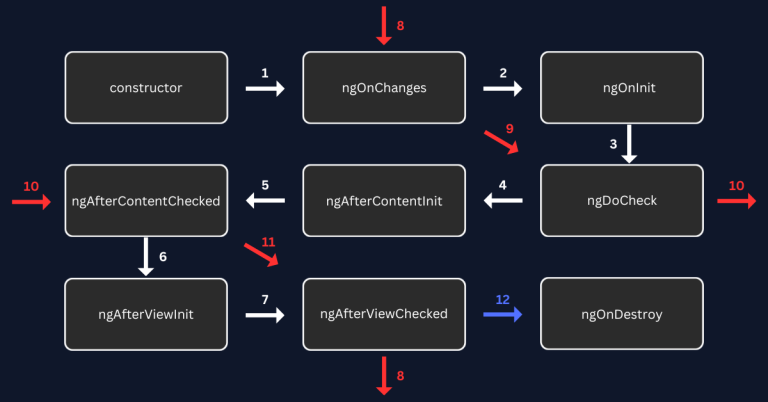
\includegraphics[width=.85\textwidth]{images/angularlifecycle.png}
	\caption[Životní cyklus Angularu]{Životní cyklus Angularu \cite{angularlifecycle}}
	\label{fig:angularlifecycle}
\end{figure}

\subsubsection{State management}

K~základní práci se stavy slouží vlastnosti třídy, které inicializujeme JavaScriptovou hodnotou. 
Do budoucna můžeme počítat s~lepší podporou signálů, které aktualizují DOM efektivněji a~rychleji. 
Pokročilejší způsob sdílení stavů v~aplikaci spočívá ve využití služeb, v~nichž uložíme stavy a~následně je sdílíme mezi komponentami.\cite{angulardev}

Pro reaktivní či asynchronní operace, nebo obecně složitější funkcionality, využijeme balíček RxJS, který je již součástí Angularu. 
RxJS poskytuje datový typ Observable, který reprezentuje data, jež se mohou měnit v~čase.\cite{angulario,rxjslibrary}

V~případě, že potřebujeme sdílet stavy globálně (mezi různými částmi aplikace), můžeme využít knihovnu NgRx, která je inspirována knihovnou Redux.\cite{angularstatemanagement,ngrxlib}

\subsubsection{Routování}

Angular poskytuje vestavěný systém routování -- konkrétně balíček @angular/router, který na straně klienta umožňuje přepínat mezi různými částmi aplikace. 
Klasické webové stránky při změně URL pokaždé žádají o~nové dokumenty. Routování na straně klienta může provést aktualizaci stránky bez dalších duplikátních dotazů. 
Při vyžádání dané cesty pak vykreslíme požadovaný obsah a~požádáme pouze o~data potřebná k~vykreslení. 
Získáme tak rychlejší uživatelskou zkušenost, jelikož prohlížeč nevyžaduje nové dokumenty a~nemusí vyhodnocovat kaskádové styly či JavaScript.

Abychom zaregistrovali cesty aplikace pomocí knihovny @angular/router, poskytneme samotný router pomocí funkce provideRouter do aplikačního nastavení. 
Routeru následně předáme pole cest aplikace. Jednotlivé obsahy stránek, které se mají zobrazit, vykreslíme pomocí elementu router-outlet.\cite{angulardev,learningangular}

\subsubsection{Ekosystém}

Angular je komplexní framework, v~němž jsou obsaženy základní balíčky všeho druhu potřebné pro vývoj webových aplikací. 
Framework se stále vyvíjí a~jeho ekosystém se neustále rozrůstá, a~to i~přes velikost projektu. 
Angular nabízí rozsáhlou kolekci balíčků třetích stran, které vývojáři využívají pro usnadnění práce s~různými částmi aplikace. 
Nechybí ani balíček @angular/cli, jenž usnadňuje vývoj aplikace, testování, aktualizaci kódu i~nasazení.\cite{angulardev,learningangular}